\newcommand{\AIONDiagramHolography}{
\begin{tikzpicture}[
    state/.style={circle, draw, fill=gray!20, minimum size=8mm, inner sep=0pt},
    boundary/.style={draw, rounded corners, thick, dashed, inner sep=6pt}
  ]
  \node[state] (u0) at (0,0) {$U_0$};
  \node[state] (u1) at (2,0) {$U_1$};
  \node[state] (u2) at (4,0) {$U_2$};
  \node[state] (un) at (6,0) {$U_n$};

  \draw[->, thick] (u0) -- (u1) node[midway, above] {\scriptsize $\mu_0$};
  \draw[->, thick] (u1) -- (u2) node[midway, above] {\scriptsize $\mu_1$};
  \draw[->, thick] (u2) -- (un) node[midway, above] {\scriptsize $\cdots$};

  \node[boundary, fit=(u0)] (b0) {};
  \node[below=2mm of b0] {\scriptsize $U_0$};

  \node[boundary, fit=(u0) (u1) (u2)] (bp) {};
  \node[below=2mm of bp] {\scriptsize payload $P$};

  \node[boundary, fit=(u0) (bp)] (b) {};
  \node[above=2mm of b] {\scriptsize boundary $(U_0,P)$};

  \draw[->, thick, dashed] (b.east) to[out=0,in=180] (un.west);
\end{tikzpicture}
}

\newcommand{\AIONDiagramWormhole}{
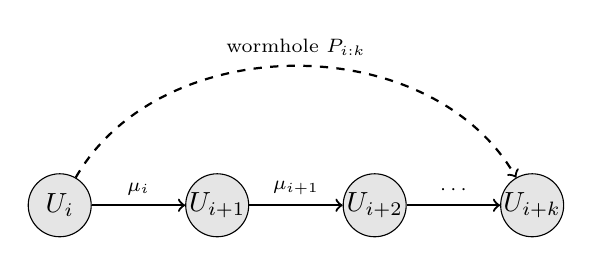
\begin{tikzpicture}[
    state/.style={circle, draw, fill=gray!20, minimum size=8mm, inner sep=0pt},
    wormhole/.style={->, thick, dashed},
    normal/.style={->, thick}
  ]
  \node[state] (u0) at (0,0) {$U_i$};
  \node[state] (u1) at (2,0) {$U_{i+1}$};
  \node[state] (u2) at (4,0) {$U_{i+2}$};
  \node[state] (uk) at (6,0) {$U_{i+k}$};

  \draw[normal] (u0) -- (u1) node[midway, above] {\scriptsize $\mu_i$};
  \draw[normal] (u1) -- (u2) node[midway, above] {\scriptsize $\mu_{i+1}$};
  \draw[normal] (u2) -- (uk) node[midway, above] {\scriptsize $\cdots$};

  \draw[wormhole] (u0) to[out=60,in=120] node[midway, above] {\scriptsize wormhole $P_{i:k}$} (uk);
\end{tikzpicture}
}

\newcommand{\AIONDiagramSlicing}{
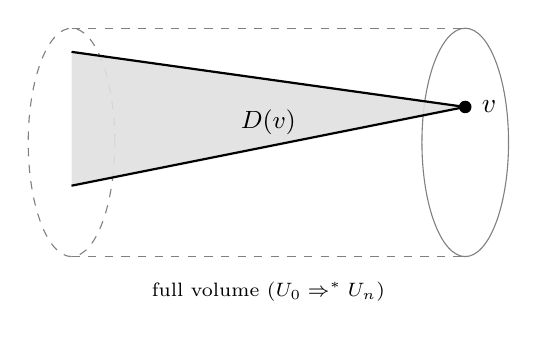
\begin{tikzpicture}
  % Bulk "volume" cylinder
  \draw[gray, dashed] (0,0) ellipse (0.55 and 1.45);
  \draw[gray] (5,0) ellipse (0.55 and 1.45);
  \draw[gray, dashed] (0,1.45) -- (5,1.45);
  \draw[gray, dashed] (0,-1.45) -- (5,-1.45);

  % Backward cone (derivation graph)
  \node[circle, fill=black, inner sep=1.6pt, label=right:$v$] (v) at (5, 0.45) {};
  \fill[black!12, opacity=0.9] (5, 0.45) -- (0, -0.55) -- (0, 1.15) -- cycle;
  \draw[black, thick] (5, 0.45) -- (0, -0.55);
  \draw[black, thick] (5, 0.45) -- (0, 1.15);

  \node at (2.5, 0.25) {\small $D(v)$};
  \node[align=center, font=\scriptsize, below] at (2.5, -1.65) {full volume ($U_0 \Rightarrow^* U_n$)};
\end{tikzpicture}
}

\newcommand{\AIONDiagramForkAndWormhole}{
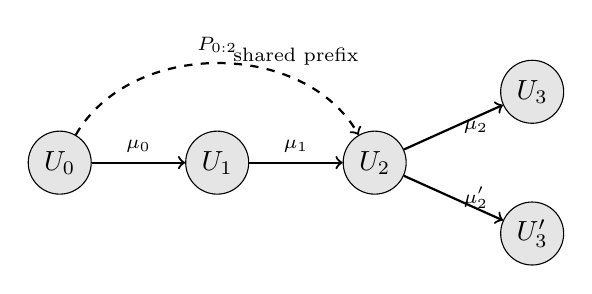
\begin{tikzpicture}[
    state/.style={circle, draw, fill=gray!20, minimum size=8mm, inner sep=0pt},
    normal/.style={->, thick},
    wormhole/.style={->, thick, dashed},
    fork/.style={->, thick}
  ]
  \node[state] (u0) at (0,0) {$U_0$};
  \node[state] (u1) at (2,0) {$U_1$};
  \node[state] (u2) at (4,0) {$U_2$};
  \node[state] (u3) at (6,0.9) {$U_3$};
  \node[state] (u3p) at (6,-0.9) {$U_3'$};

  % Full (uncompressed) prefix
  \draw[normal] (u0) -- (u1) node[midway, above] {\scriptsize $\mu_0$};
  \draw[normal] (u1) -- (u2) node[midway, above] {\scriptsize $\mu_1$};

  % Wormhole compression of the prefix
  \draw[wormhole] (u0) to[out=60,in=120] node[midway, above] {\scriptsize $P_{0:2}$} (u2);

  % Fork at next tick
  \draw[fork] (u2) -- (u3) node[midway, right] {\scriptsize $\mu_2$};
  \draw[fork] (u2) -- (u3p) node[midway, right] {\scriptsize $\mu_2'$};

  \node[font=\scriptsize] at (3,1.35) {shared prefix};
\end{tikzpicture}
}
